%%%%%%%%%%%%%%%%%%%%%%%%
%
% $Autor: Hemanth Jadiswami Prabhakaran $
% $Datum: 2025-06-30 11:18:51Z $
% $Pfad: GitHub/BA25-01-Time-Series/Manual/Chapters/en/04GUIAndUserInterface.tex $
% $Version: 1 $
%
% $Project: BA25-Time-Series $
%
%%%%%%%%%%%%%%%%%%%%%%%%



\chapter{GUI and User Interface Documentation}

\section{Interface Design Philosophy}

The Walmart Sales Forecasting System employs a user-centric design approach built on the Streamlit framework. Both applications feature intuitive, web-based interfaces designed to minimize the learning curve while providing comprehensive functionality for time series forecasting.

\begin{figure}[H]
    \centering
    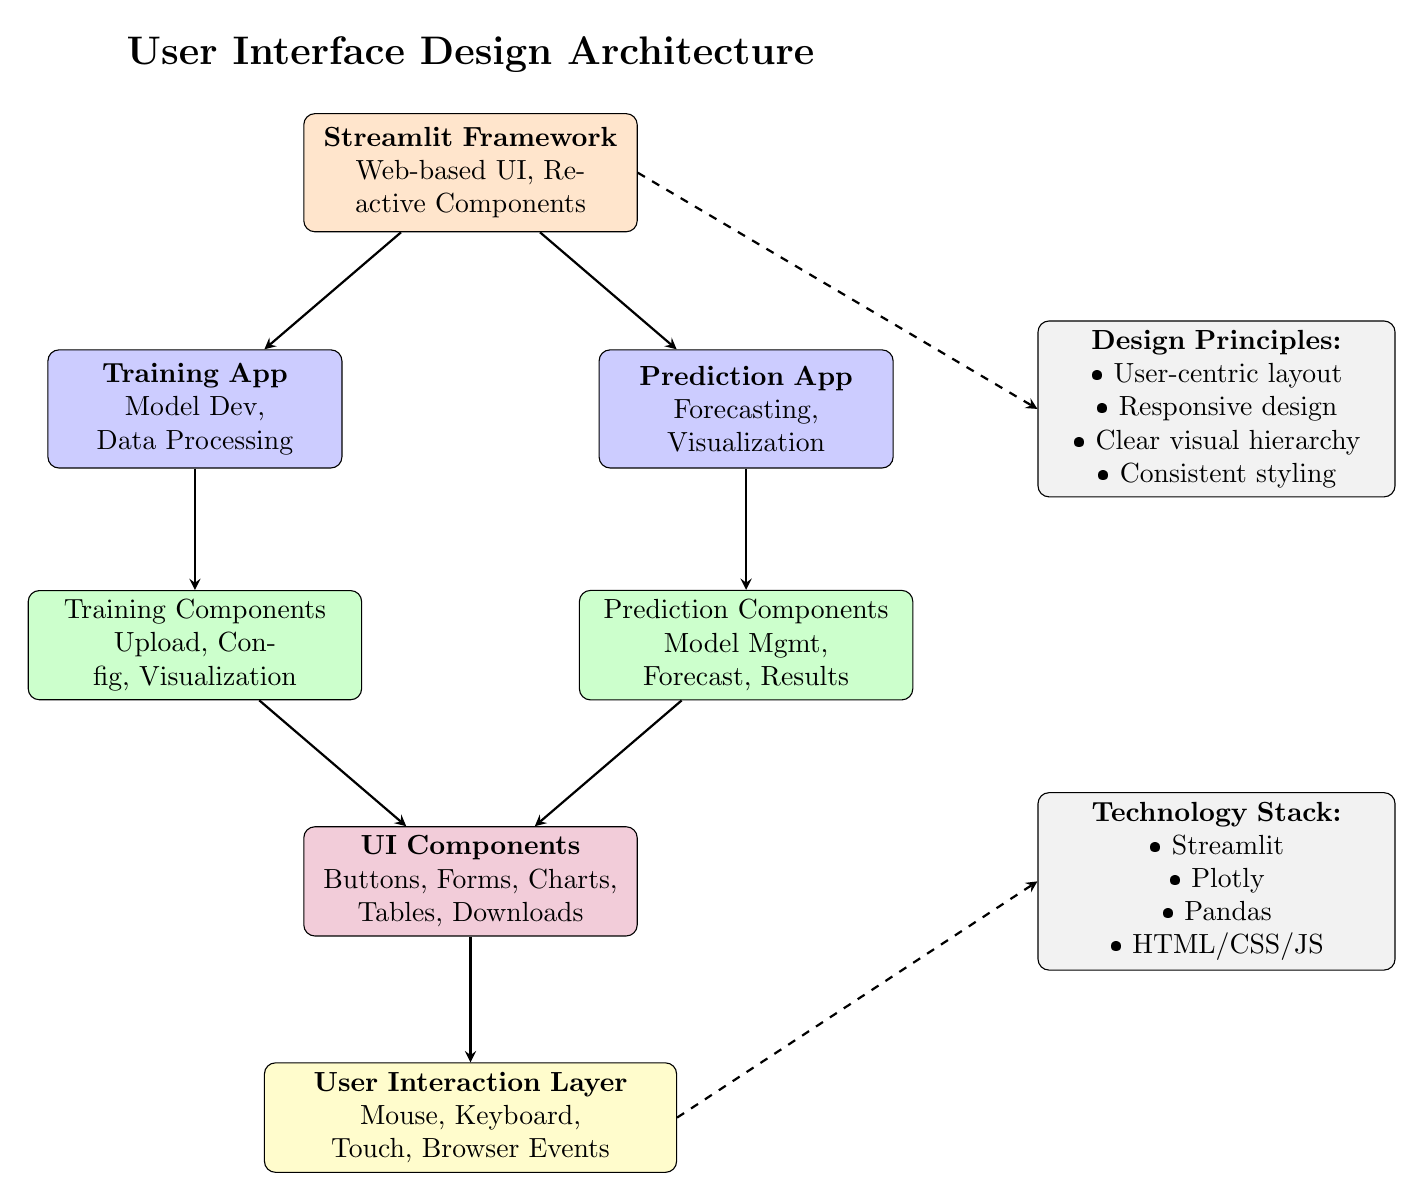
\begin{tikzpicture}[
	layer/.style={rectangle, draw, fill=blue!20, text width=3.5cm, text centered, rounded corners, minimum height=1.5cm},
	component/.style={rectangle, draw, fill=green!20, text width=4cm, text centered, rounded corners, minimum height=1.2cm},
	framework/.style={rectangle, draw, fill=orange!20, text width=4cm, text centered, rounded corners, minimum height=1.5cm},
	ui/.style={rectangle, draw, fill=purple!20, text width=4cm, text centered, rounded corners, minimum height=1.2cm},
	user/.style={rectangle, draw, fill=yellow!20, text width=5cm, text centered, rounded corners, minimum height=1.2cm},
	box/.style={rectangle, draw, fill=gray!10, text width=4.3cm, text centered, rounded corners, minimum height=1.2cm},
	arrow/.style={thick,->,>=stealth}
	]
	
	% Title
	\node at (0,13.5) {\Large\textbf{User Interface Design Architecture}};
	
	% Framework Layer
	\node[framework] (streamlit) at (0,12) {\textbf{Streamlit Framework}\\Web-based UI, Reactive Components};
	
	% Application Layer
	\node[layer] (training_app) at (-3.5,9) {\textbf{Training App}\\Model Dev, Data Processing};
	\node[layer] (prediction_app) at (3.5,9) {\textbf{Prediction App}\\Forecasting, Visualization};
	
	% Components Layer
	\node[component] (training_comp) at (-3.5,6) {Training Components\\Upload, Config, Visualization};
	\node[component] (prediction_comp) at (3.5,6) {Prediction Components\\Model Mgmt, Forecast, Results};
	
	% UI Elements (combined)
	\node[ui] (ui_components) at (0,3) {\textbf{UI Components}\\Buttons, Forms, Charts, Tables, Downloads};
	
	% User Interaction
	\node[user] (user_layer) at (0,0) {\textbf{User Interaction Layer}\\Mouse, Keyboard, Touch, Browser Events};
	
	% Arrows - Framework to Apps
	\draw[arrow] (streamlit) -- (training_app);
	\draw[arrow] (streamlit) -- (prediction_app);
	
	% Arrows - Apps to Components
	\draw[arrow] (training_app) -- (training_comp);
	\draw[arrow] (prediction_app) -- (prediction_comp);
	
	% Arrows - Components to UI
	\draw[arrow] (training_comp) -- (ui_components);
	\draw[arrow] (prediction_comp) -- (ui_components);
	
	% Arrows - UI to User
	\draw[arrow] (ui_components) -- (user_layer);
	
	% Side Boxes
	\node[box, anchor=west] (principles) at (7.2,9) {
		\textbf{Design Principles:}\\
		• User-centric layout\\
		• Responsive design\\
		• Clear visual hierarchy\\
		• Consistent styling
	};
	
	\node[box, anchor=west] (stack) at (7.2,3) {
		\textbf{Technology Stack:}\\
		• Streamlit\\
		• Plotly\\
		• Pandas\\
		• HTML/CSS/JS
	};
	
	% Dashed side arrows
	\draw[arrow, dashed] (streamlit.east) -- (principles.west);
	\draw[arrow, dashed] (user_layer.east) -- (stack.west);
	
\end{tikzpicture}
    \caption{User Interface Design Architecture}
    \label{fig:interface_design}
\end{figure}

\section{Training Application Interface}

\subsection{Main Navigation Structure}

The Training Application organizes functionality into logical sections with clear visual hierarchy:

\begin{figure}[H]
    \centering
    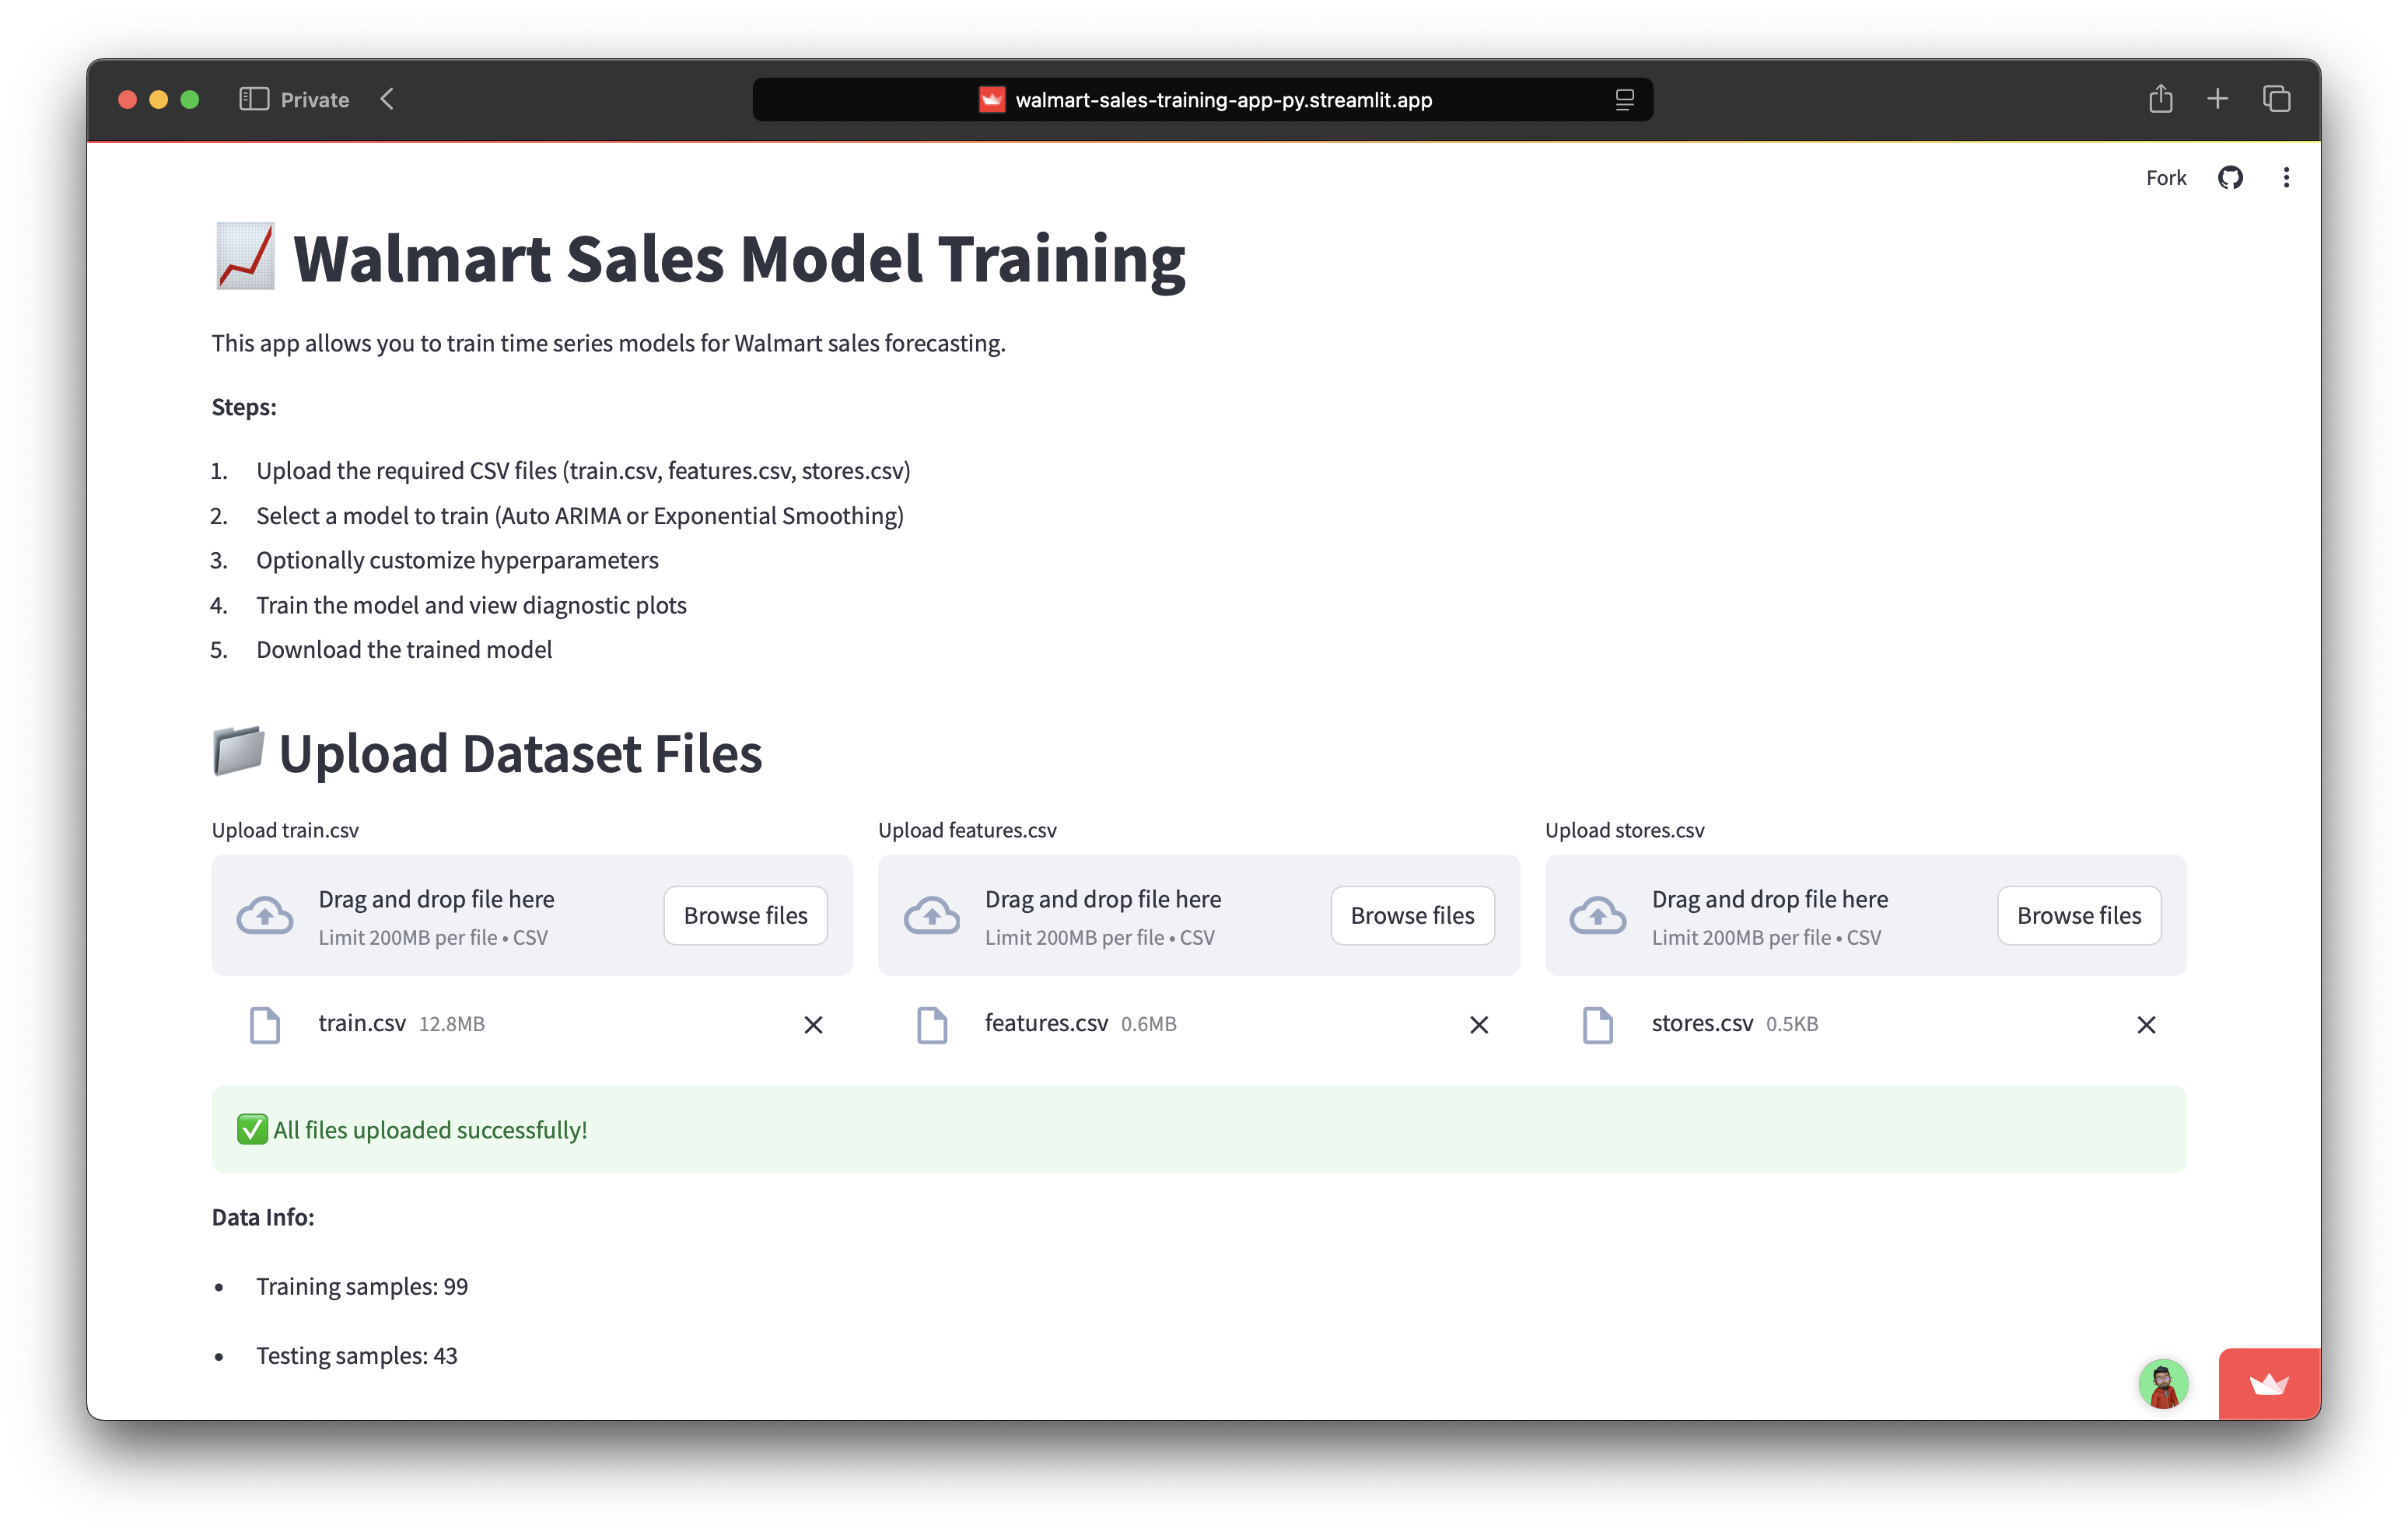
\includegraphics[width=0.9\textwidth]{Images/04GUIAndUserInterface/TrainingAppOverview.png}
    \caption{Training Application Complete Interface Overview}
    \label{fig:training_app_overview}
\end{figure}

\subsection{Header Section}

\textbf{Application Title and Description}
\begin{itemize}
    \item \textbf{Main Title}: " Walmart Sales Model Training"
    \item \textbf{Subtitle}: Comprehensive description of training capabilities
    \item \textbf{Step-by-Step Guide}: Visual workflow overview for new users
\end{itemize}

\begin{figure}[H]
    \centering
    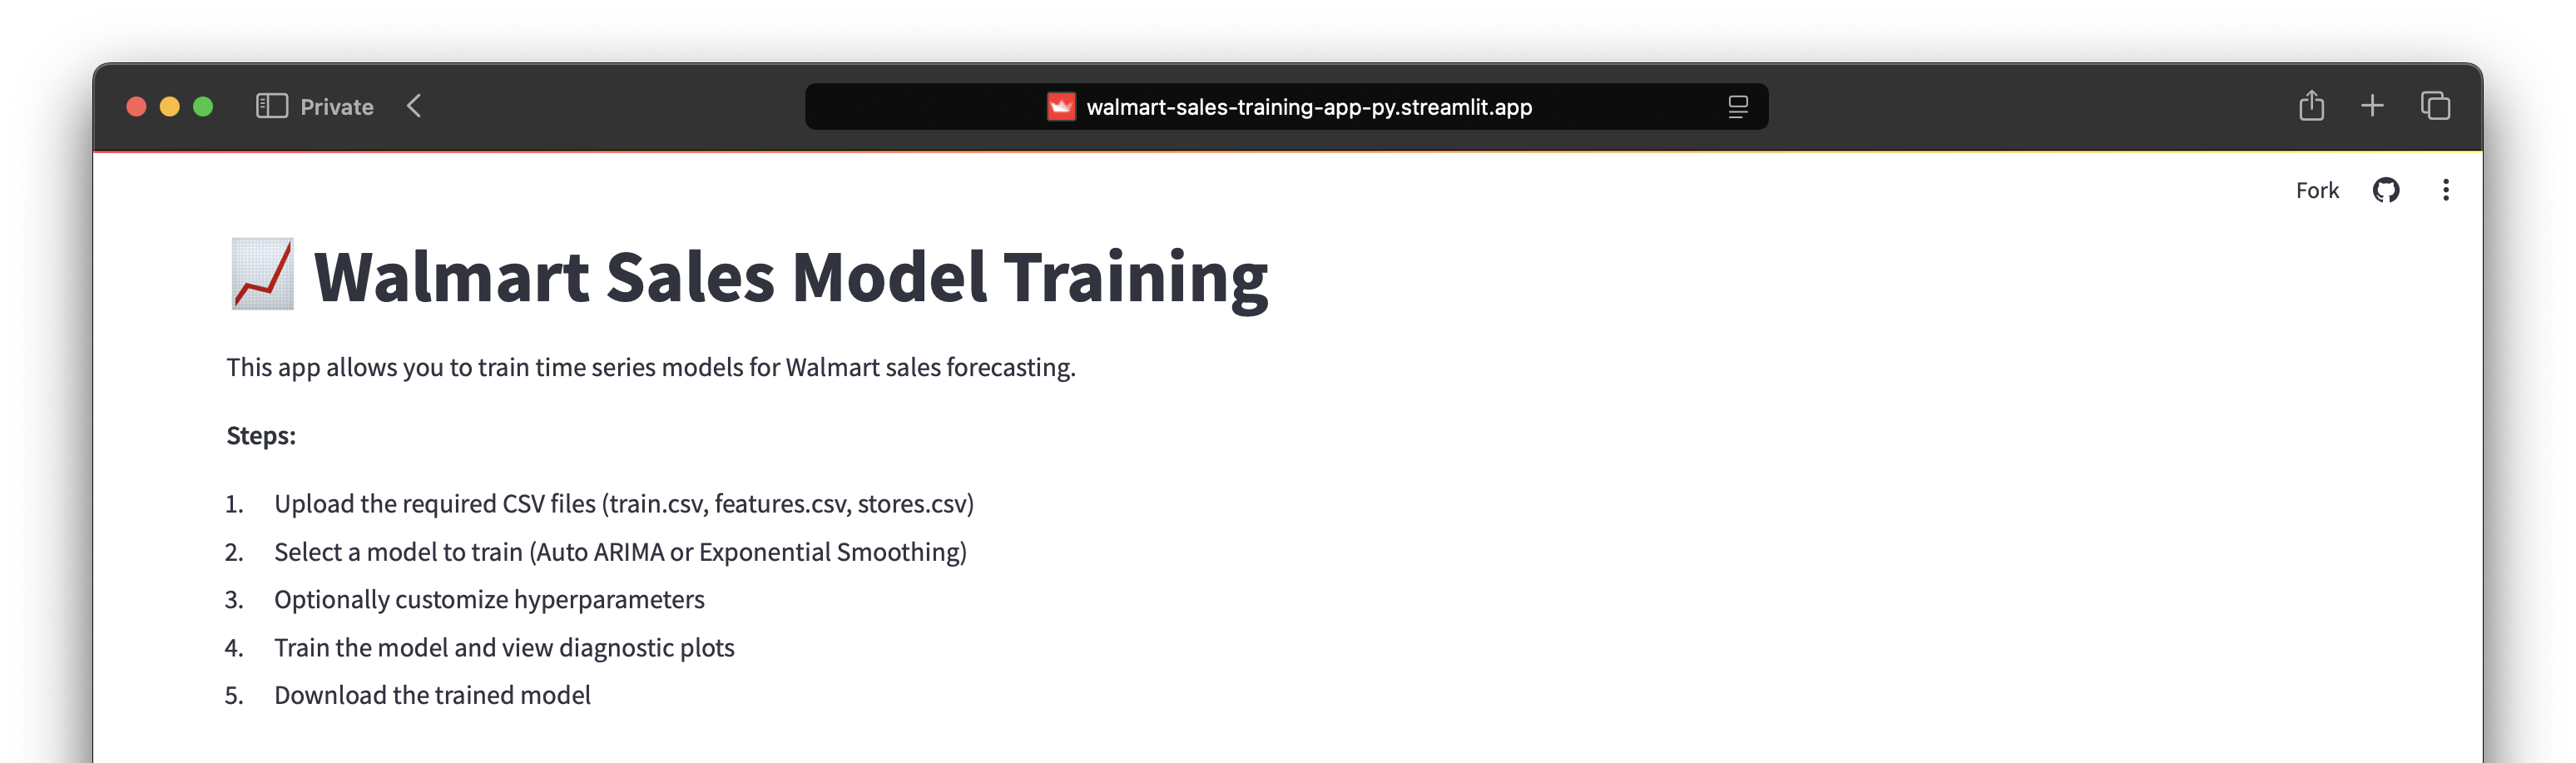
\includegraphics[width=0.9\textwidth]{Images/04GUIAndUserInterface/TrainingHeader.png}
    \caption{Training Application Header and Introduction}
    \label{fig:training_header}
\end{figure}

\subsection{File Upload Section}

\textbf{Multi-File Upload Interface}

The data upload section uses a three-column layout for required CSV files:

\begin{itemize}
    \item \textbf{Column 1}: train.csv uploader with drag-and-drop support
    \item \textbf{Column 2}: features.csv uploader with file validation
    \item \textbf{Column 3}: stores.csv uploader with format checking
\end{itemize}

\textbf{Visual Feedback}
\begin{itemize}
    \item \textbf{Success Indicator}: Green checkmark and " All files uploaded successfully!"
    \item \textbf{Progress Display}: Real-time upload progress bars
    \item \textbf{Error Messages}: Clear warnings for invalid file formats
\end{itemize}

\begin{figure}[H]
    \centering
    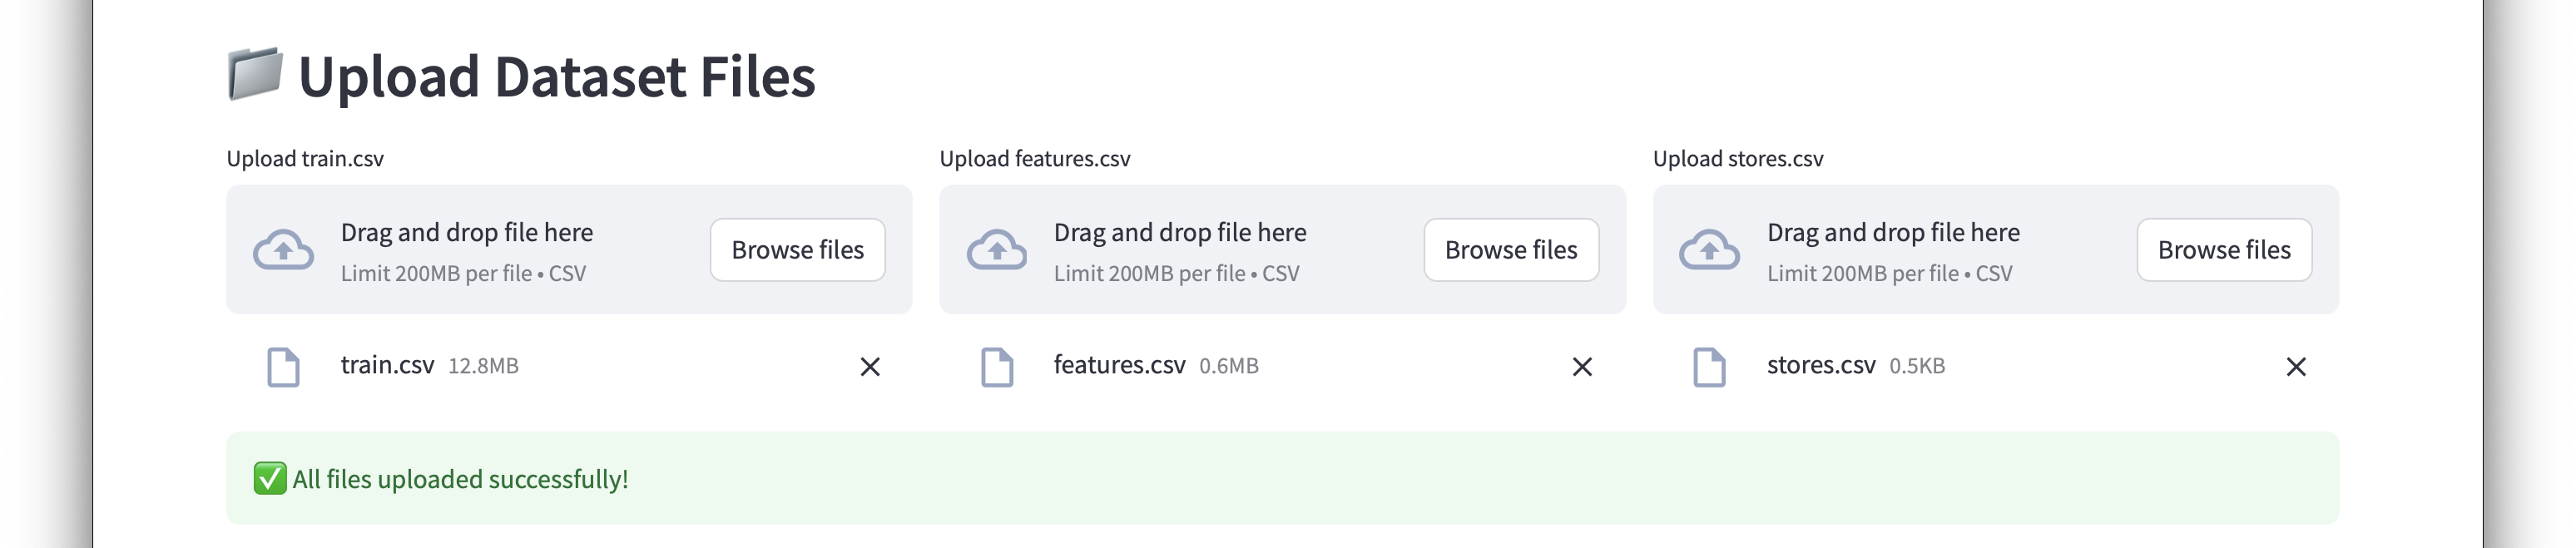
\includegraphics[width=0.9\textwidth]{Images/04GUIAndUserInterface/FileUpload.png}
    \caption{File Upload Interface with Multi-Column Layout}
    \label{fig:file_upload}
\end{figure}

\subsection{Model Selection Interface}

\textbf{Algorithm Choice Dropdown}

The model selection uses an intuitive dropdown with clear descriptions:

\begin{itemize}
    \item \textbf{Auto ARIMA}: Automatic parameter selection with seasonal components
    \item \textbf{Exponential Smoothing (Holt-Winters)}: Triple exponential smoothing
\end{itemize}

\begin{figure}[H]
    \centering
    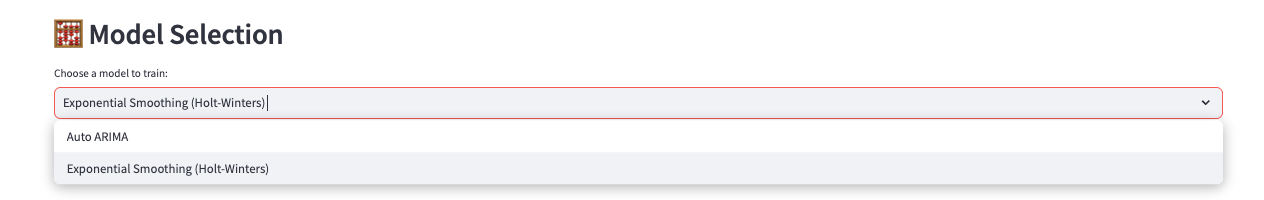
\includegraphics[width=0.9\textwidth]{Images/04GUIAndUserInterface/ModelSelection.png}
    \caption{Model Selection Dropdown Interface}
    \label{fig:model_selection}
\end{figure}

\subsection{Hyperparameter Configuration}

\textbf{Dynamic Parameter Interface}

The hyperparameter section adapts based on selected model type:

\subsubsection{Auto ARIMA Parameters}
\begin{itemize}
    \item \textbf{Left Column}: Basic ARIMA parameters (start\_p, start\_q, max\_p, max\_q)
    \item \textbf{Right Column}: Seasonal parameters (start\_P, start\_Q, max\_P, max\_Q)
    \item \textbf{Input Validation}: Numeric inputs with min/max constraints
\end{itemize}

\subsubsection{Exponential Smoothing Parameters}
\begin{itemize}
    \item \textbf{Left Column}: Smoothing parameters (seasonal\_periods, seasonal type)
    \item \textbf{Right Column}: Trend parameters (trend type, damped option)
    \item \textbf{Interactive Controls}: Dropdowns and checkboxes for easy configuration
\end{itemize}

\begin{figure}[H]
    \centering
    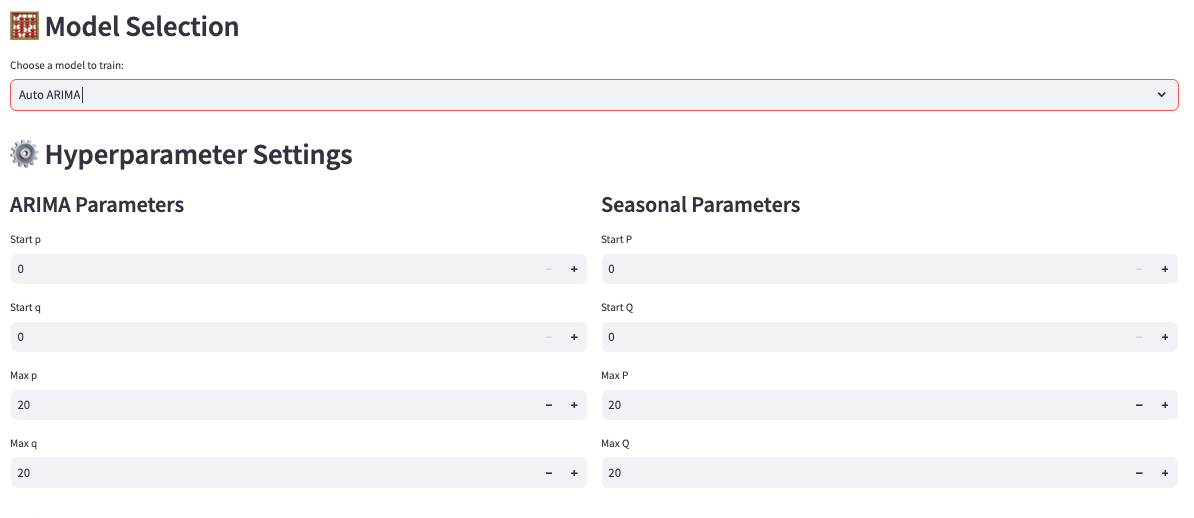
\includegraphics[width=0.9\textwidth]{Images/04GUIAndUserInterface/HyperparameterConfigArima.png}
    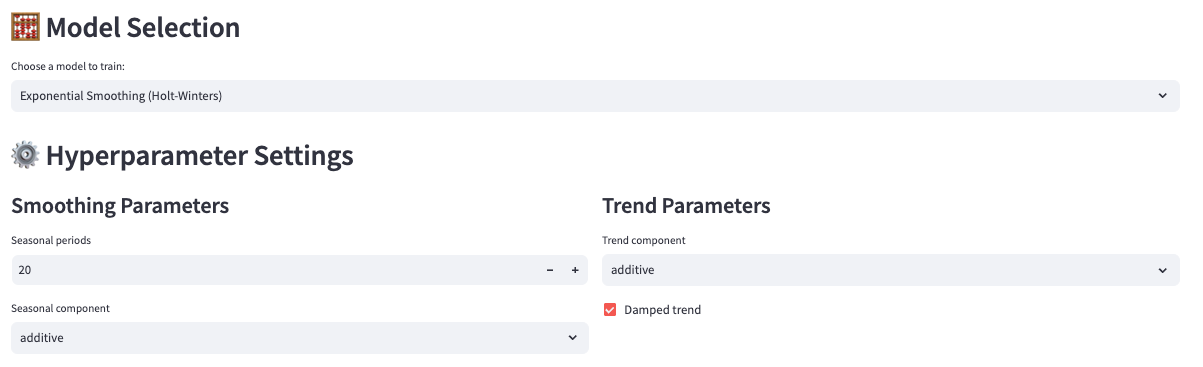
\includegraphics[width=0.9\textwidth]{Images/04GUIAndUserInterface/HyperparameterConfigETS.png}
    \caption{Dynamic Hyperparameter Configuration Interface}
    \label{fig:hyperparameter_config}
\end{figure}

\subsection{Training Execution Interface}

\textbf{Training Control and Progress}

\begin{itemize}
    \item \textbf{Primary Action Button}: Large "Start Training" button with distinctive styling
    \item \textbf{Progress Indicator}: Animated spinner with status text during training
    \item \textbf{Status Updates}: Real-time feedback on training completion
\end{itemize}

\begin{figure}[H]
    \centering
   
\includegraphics[width=0.9\textwidth]{Images/04GUIAndUserInterface/TrainingExecutionlnProgress.png}
     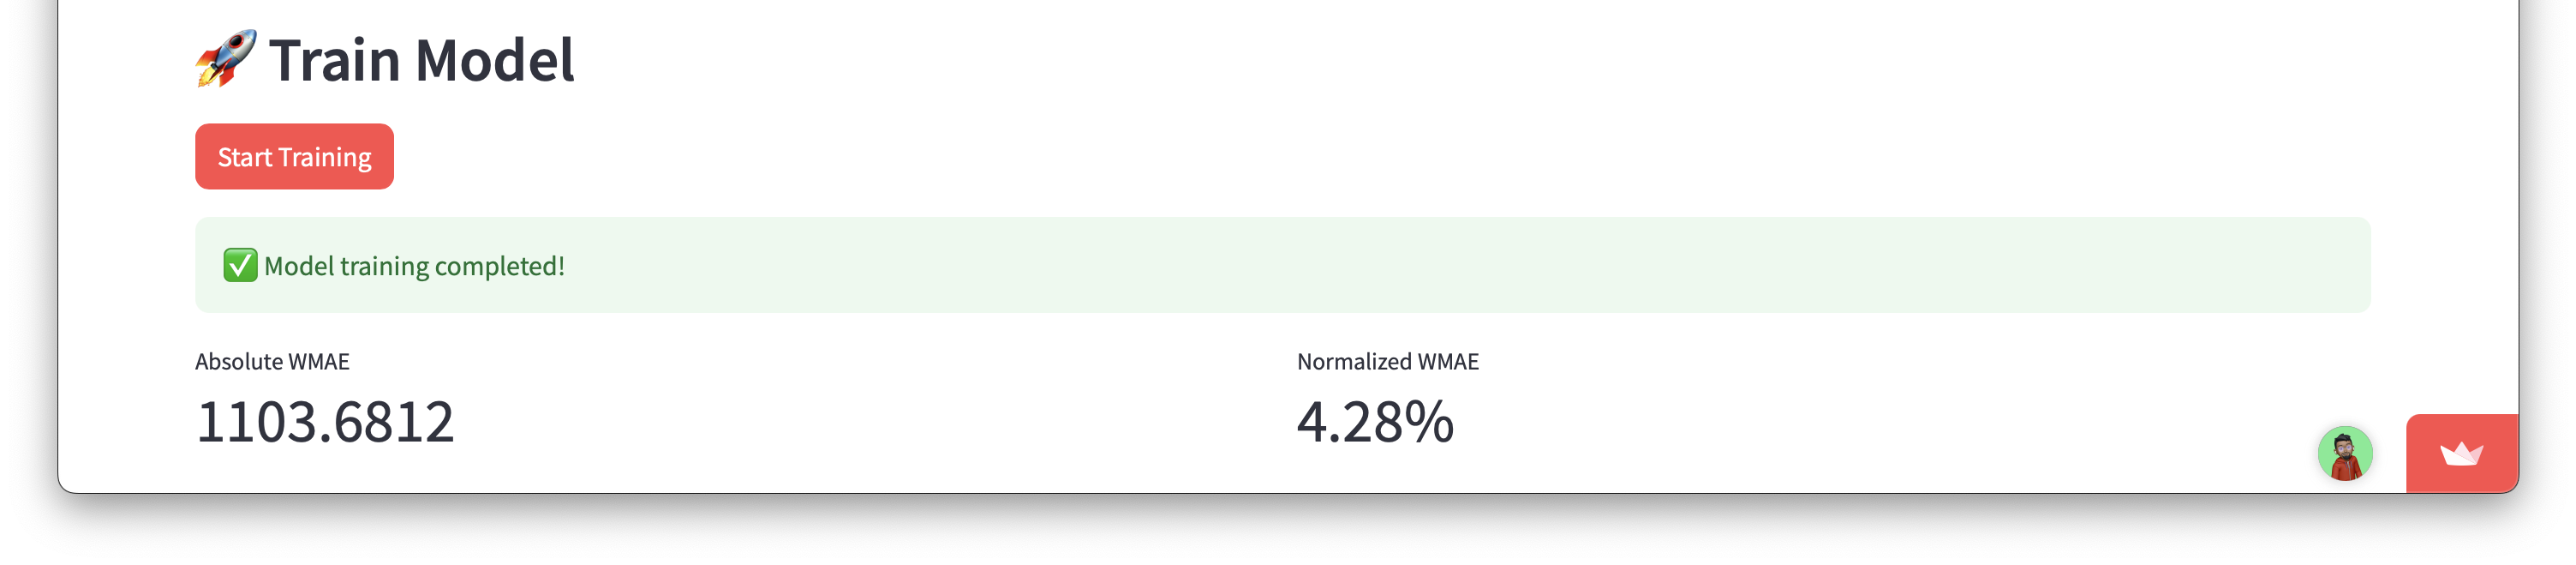
\includegraphics[width=0.9\textwidth]{Images/04GUIAndUserInterface/TrainingExecutionCompleted.png}
    \caption{Training Execution and Progress Interface}
    \label{fig:training_execution}
\end{figure}

\subsection{Results Display Interface}

\textbf{Comprehensive Results Presentation}

\begin{itemize}
    \item \textbf{Performance Metrics}: WMAE scores with color-coded interpretation
    \item \textbf{Diagnostic Plots}: Interactive matplotlib charts with training/testing visualization
    \item \textbf{Model Download}: Direct download button for trained models
    \item \textbf{Performance Guide}: Interpretive text for WMAE scores
\end{itemize}

\begin{figure}[H]
    \centering
    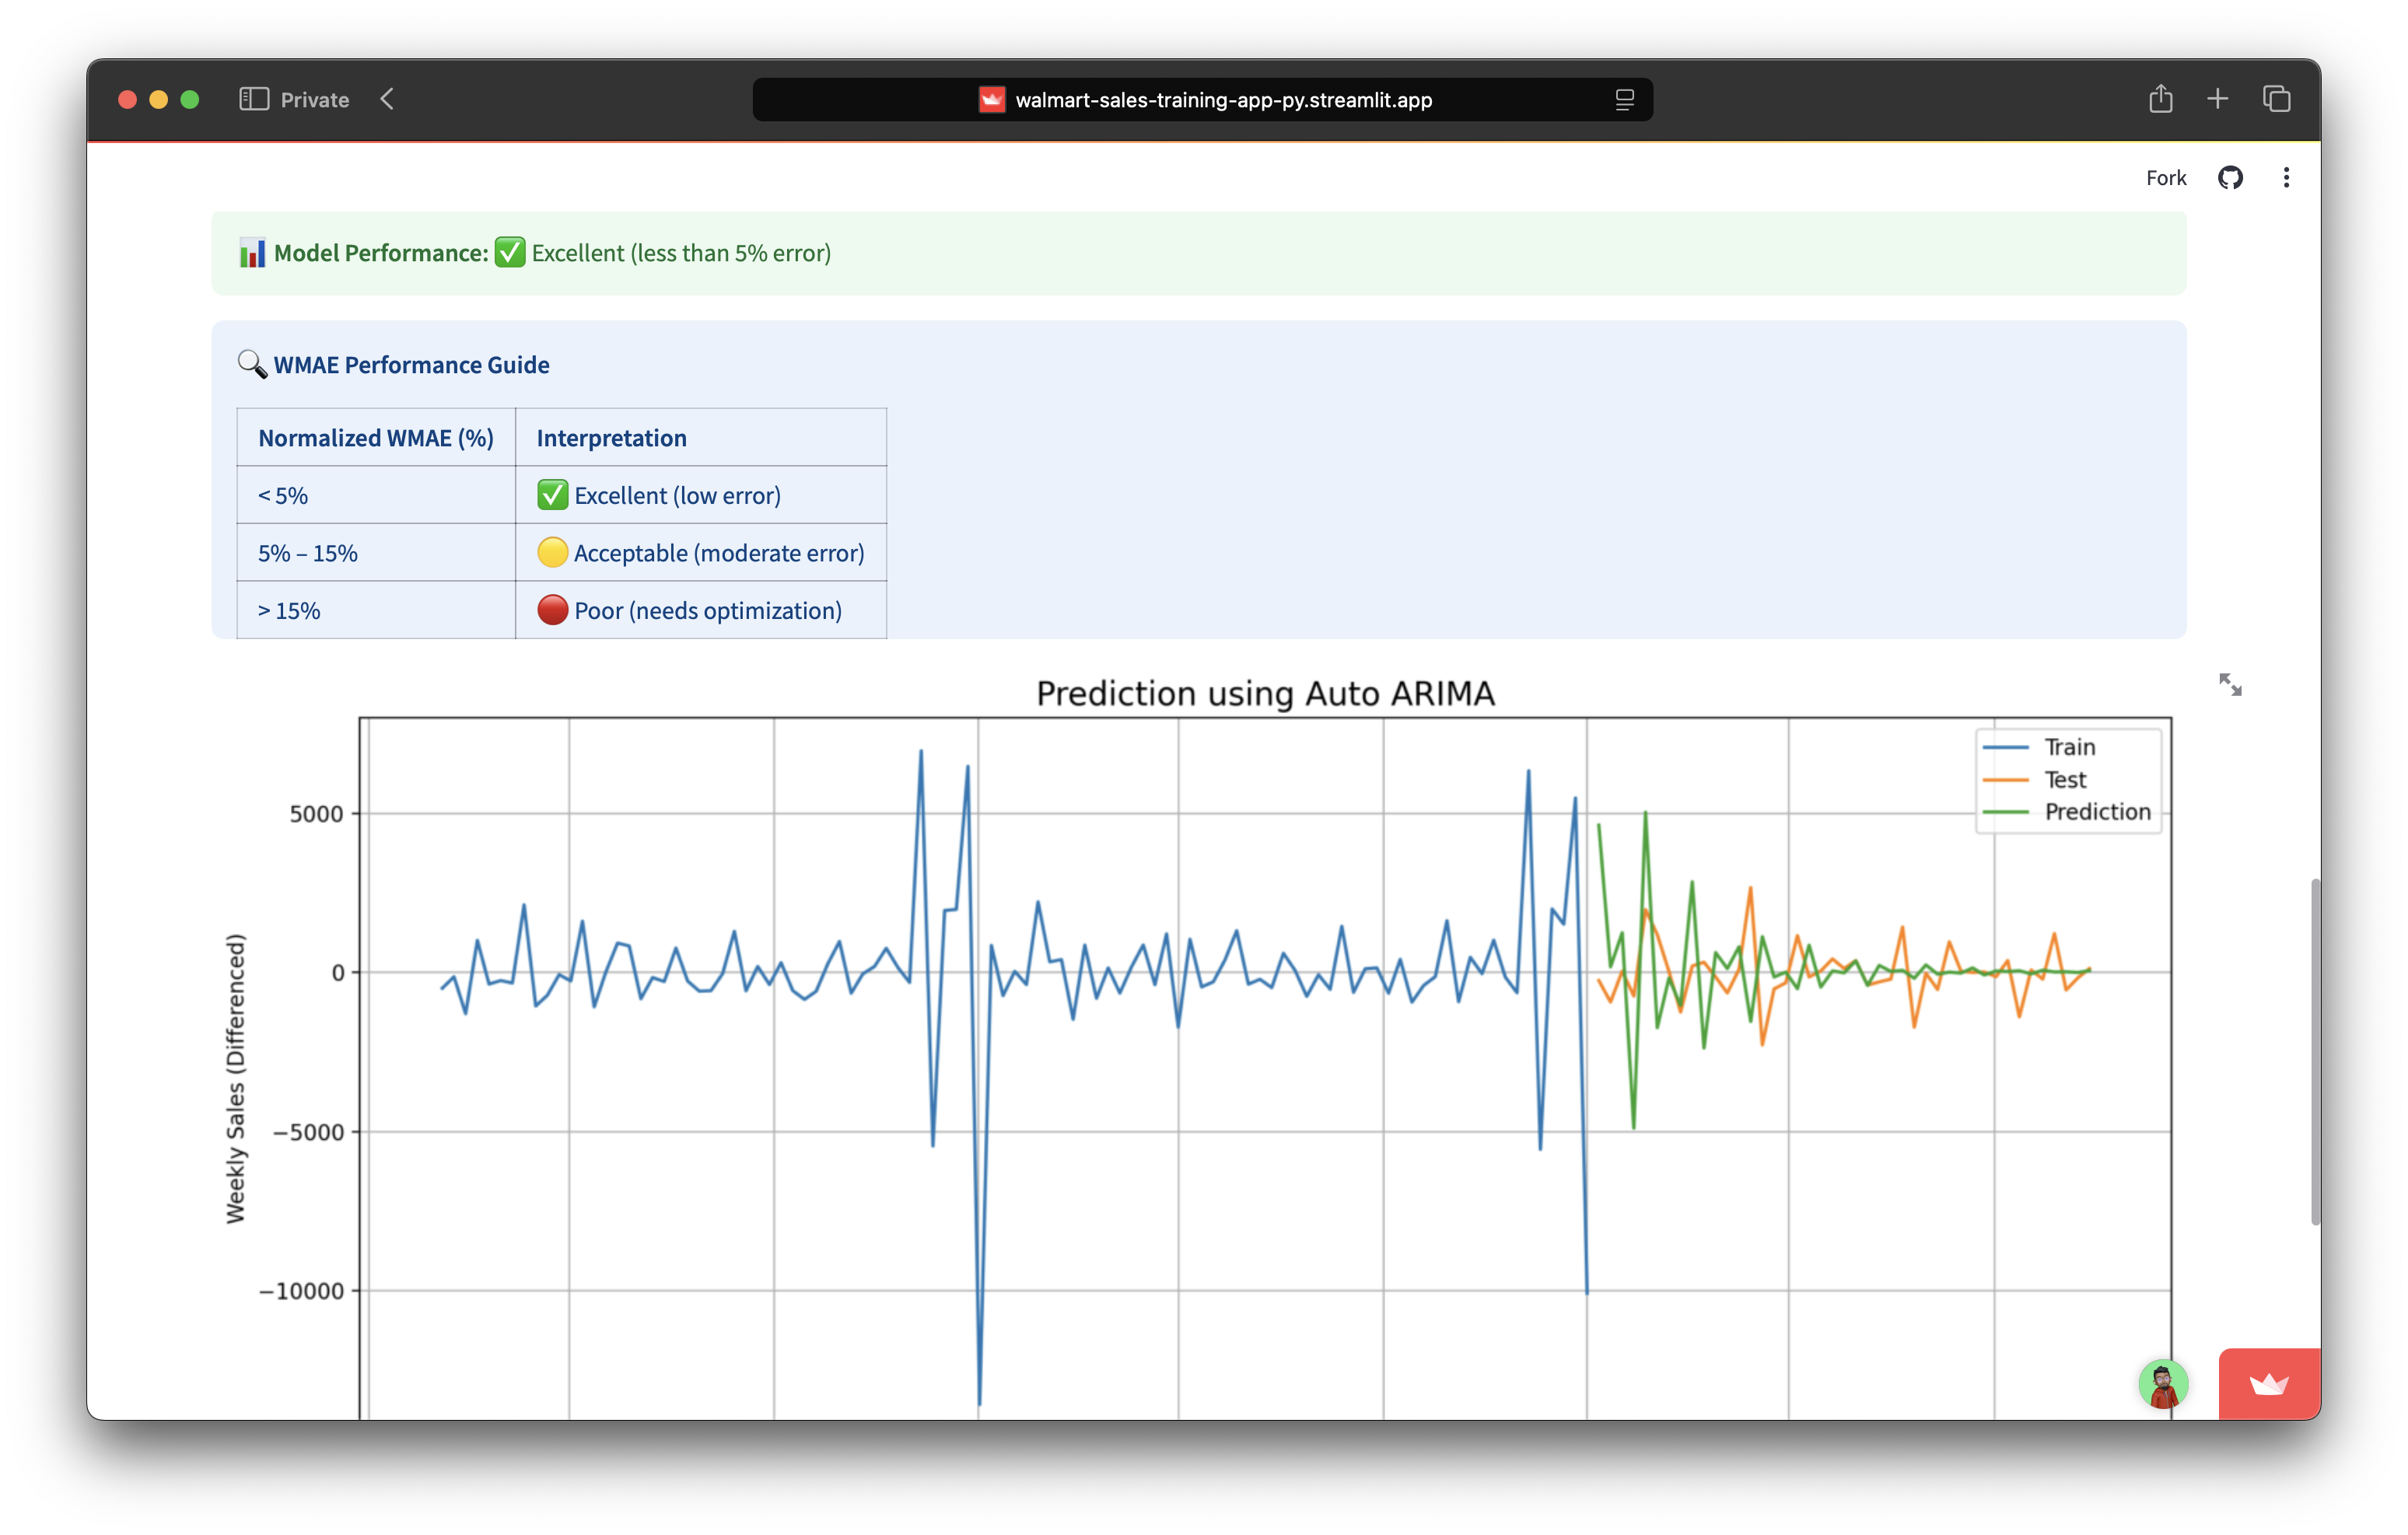
\includegraphics[width=0.9\textwidth]{Images/04GUIAndUserInterface/TrainingResults.png}
   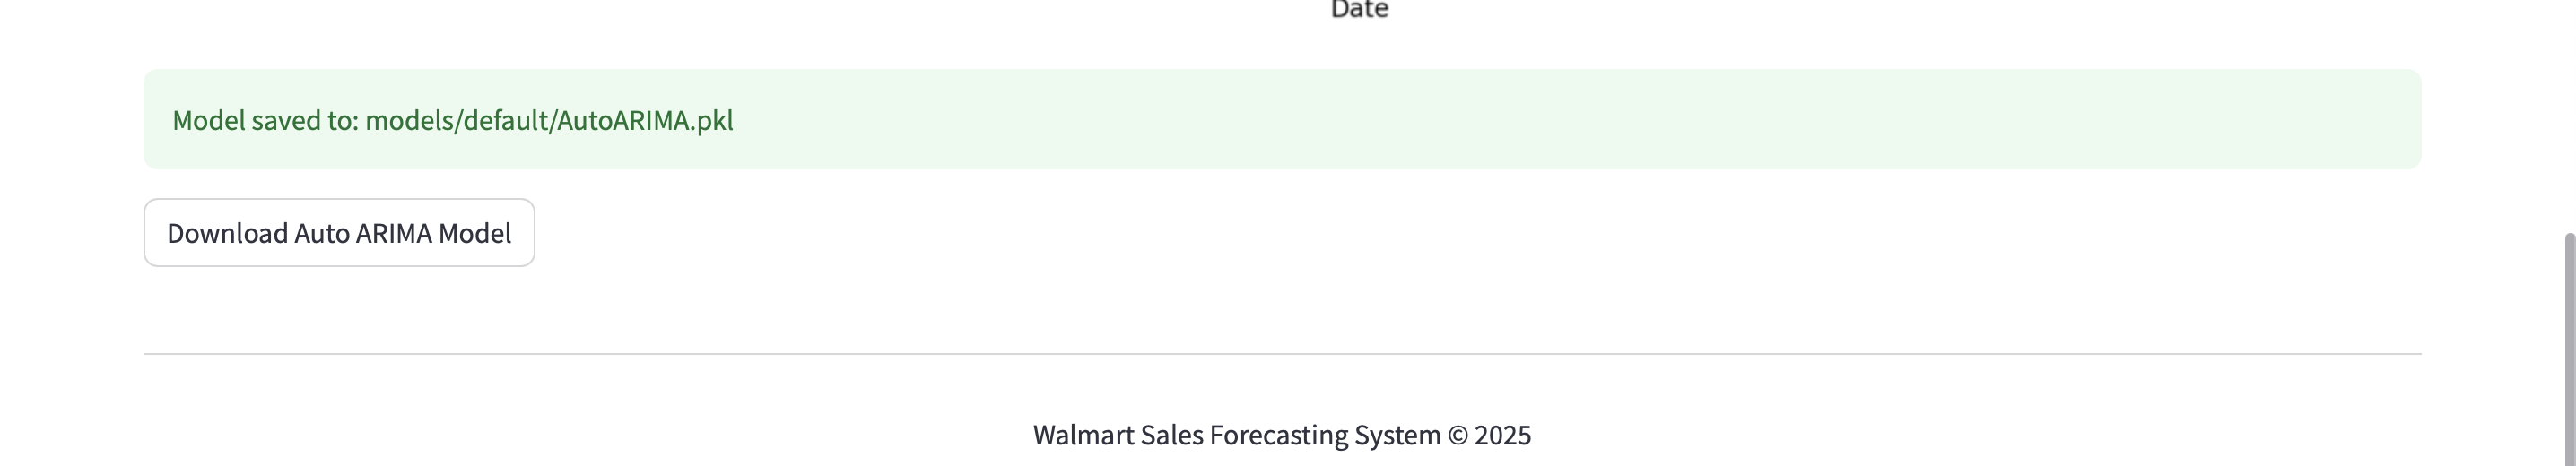
\includegraphics[width=0.9\textwidth]{Images/04GUIAndUserInterface/TrainedModelDownload.png}
     \caption{Training Results Display with Performance Metrics}
    \label{fig:training_results}
\end{figure}

\section{Prediction Application Interface}

\subsection{Main Interface Layout}

The Prediction Application emphasizes simplicity and immediate usability:

\begin{figure}[H]
    \centering
    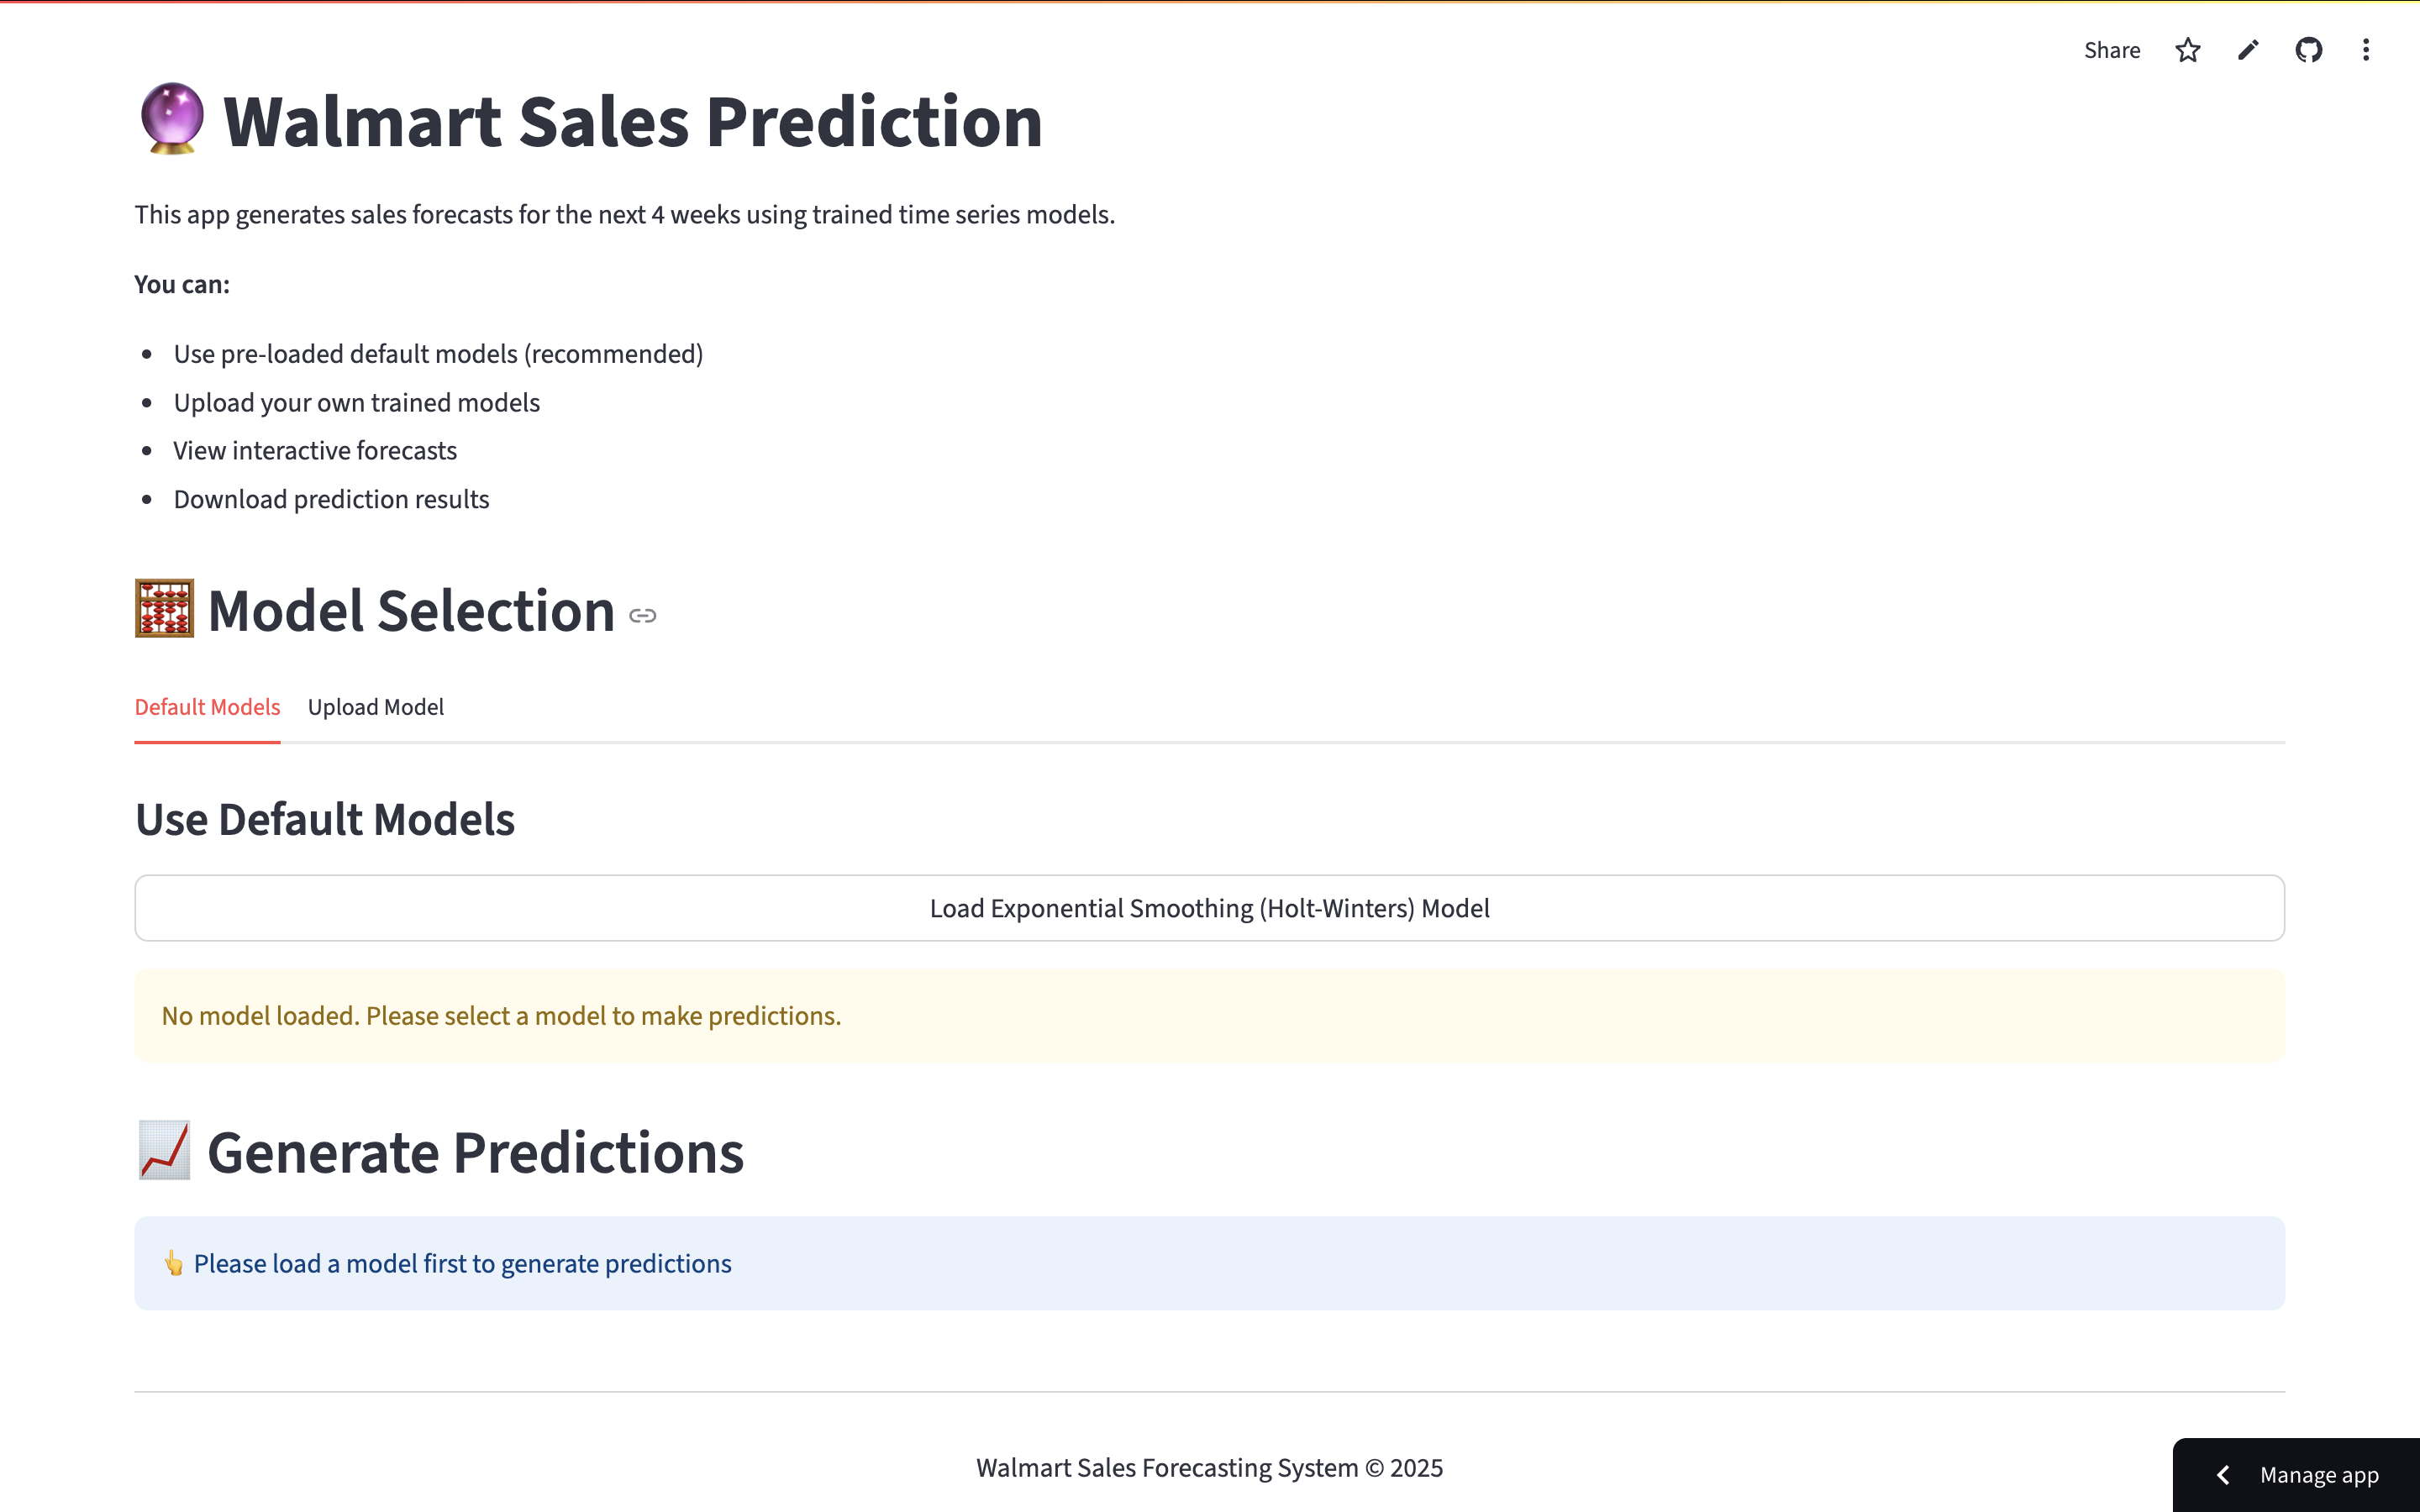
\includegraphics[width=0.9\textwidth]{Images/04GUIAndUserInterface/PredictionAppOverview.png}
    \caption{Prediction Application Complete Interface Overview}
    \label{fig:prediction_app_overview}
\end{figure}

\subsection{Application Header}

\textbf{Welcome and Introduction}
\begin{itemize}
    \item \textbf{Main Title}: " Walmart Sales Prediction" with distinctive icon
    \item \textbf{Feature Overview}: Bullet-pointed capability summary
    \item \textbf{Quick Start Guide}: Essential information for new users
\end{itemize}

\begin{figure}[H]
    \centering
    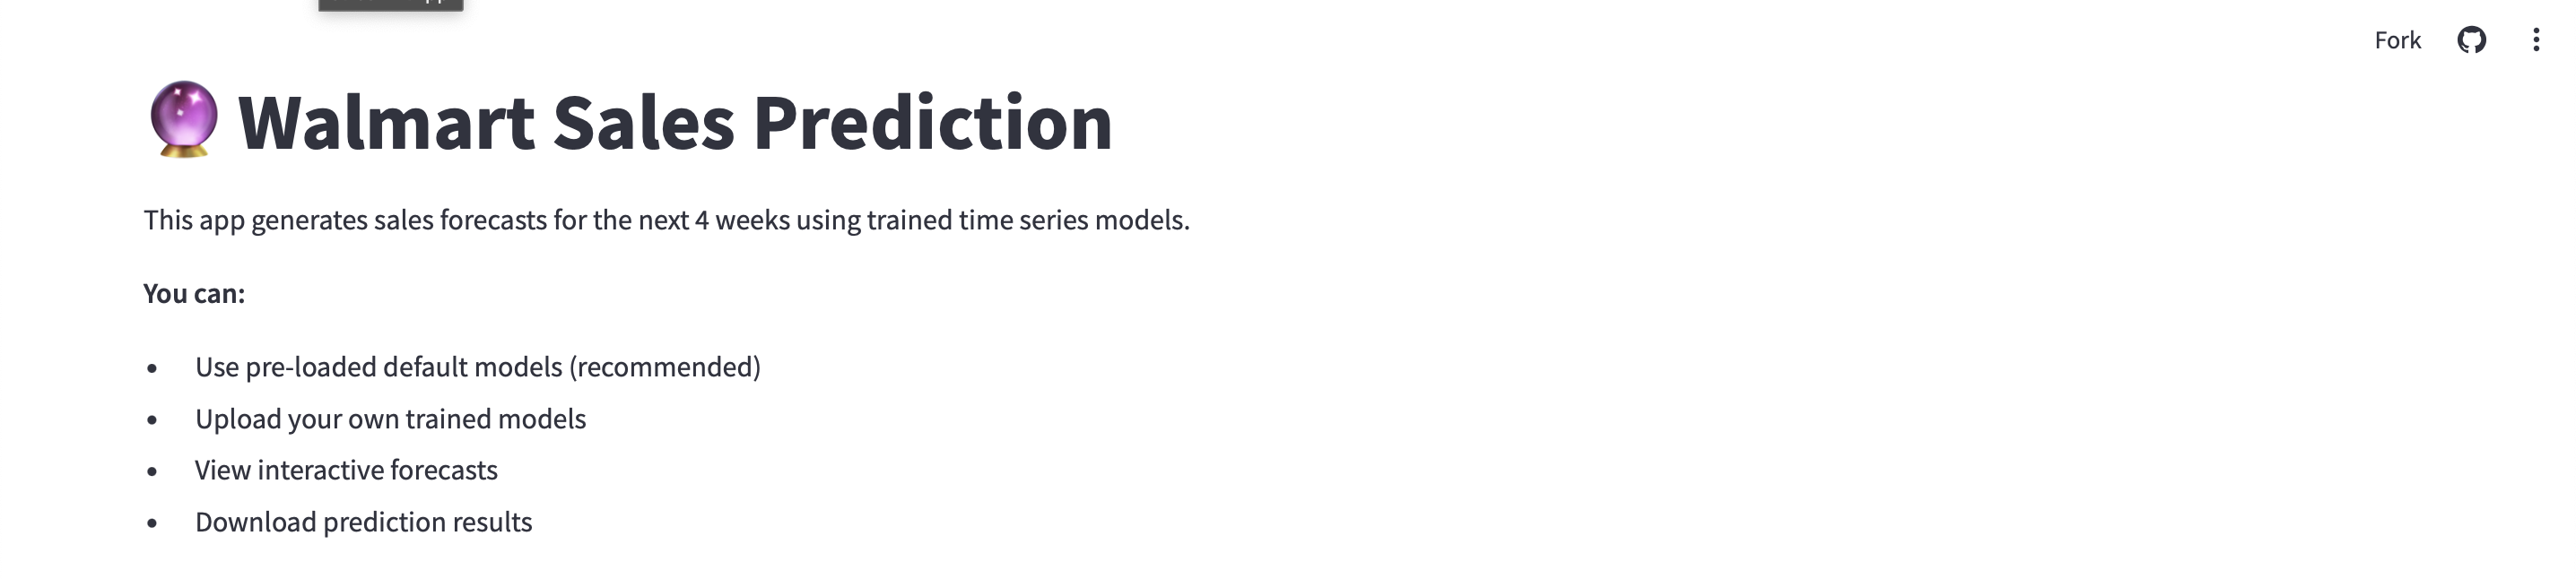
\includegraphics[width=0.9\textwidth]{Images/04GUIAndUserInterface/PredictionHeader.png}
    \caption{Prediction Application Header and Welcome Section}
    \label{fig:prediction_header}
\end{figure}

\subsection{Model Selection Tabs}

\textbf{Tabbed Interface for Model Sources}

The model selection uses clean tabs for different model sources:

\subsubsection{Default Models Tab}
\begin{itemize}
    \item \textbf{Pre-loaded Options}: Exponential Smoothing (Holt-Winters) with performance metrics
    \item \textbf{Load Button}: Full-width button with clear loading action
    \item \textbf{Performance Display}: WMAE scores and accuracy ratings
\end{itemize}

\subsubsection{Upload Model Tab}
\begin{itemize}
    \item \textbf{Model Type Selection}: Dropdown for algorithm specification
    \item \textbf{File Uploader}: Drag-and-drop interface for .pkl files
    \item \textbf{Load Button}: Context-sensitive activation based on file selection
\end{itemize}

\begin{figure}[H]
    \centering
    
\includegraphics[width=0.9\textwidth]{Images/04GUIAndUserInterface/ModelTabs.png}
    \caption{Model Selection Tabbed Interface}
    \label{fig:model_tabs}
\end{figure}

\subsection{Current Model Status}

\textbf{Active Model Information Display}

\begin{itemize}
    \item \textbf{Model Info Box}: Colored information panel showing loaded model
    \item \textbf{Model Details}: Type, source (Default/Uploaded), and performance metrics
    \item \textbf{Status Indicators}: Visual confirmation of model readiness
\end{itemize}

\begin{figure}[H]
    \centering
    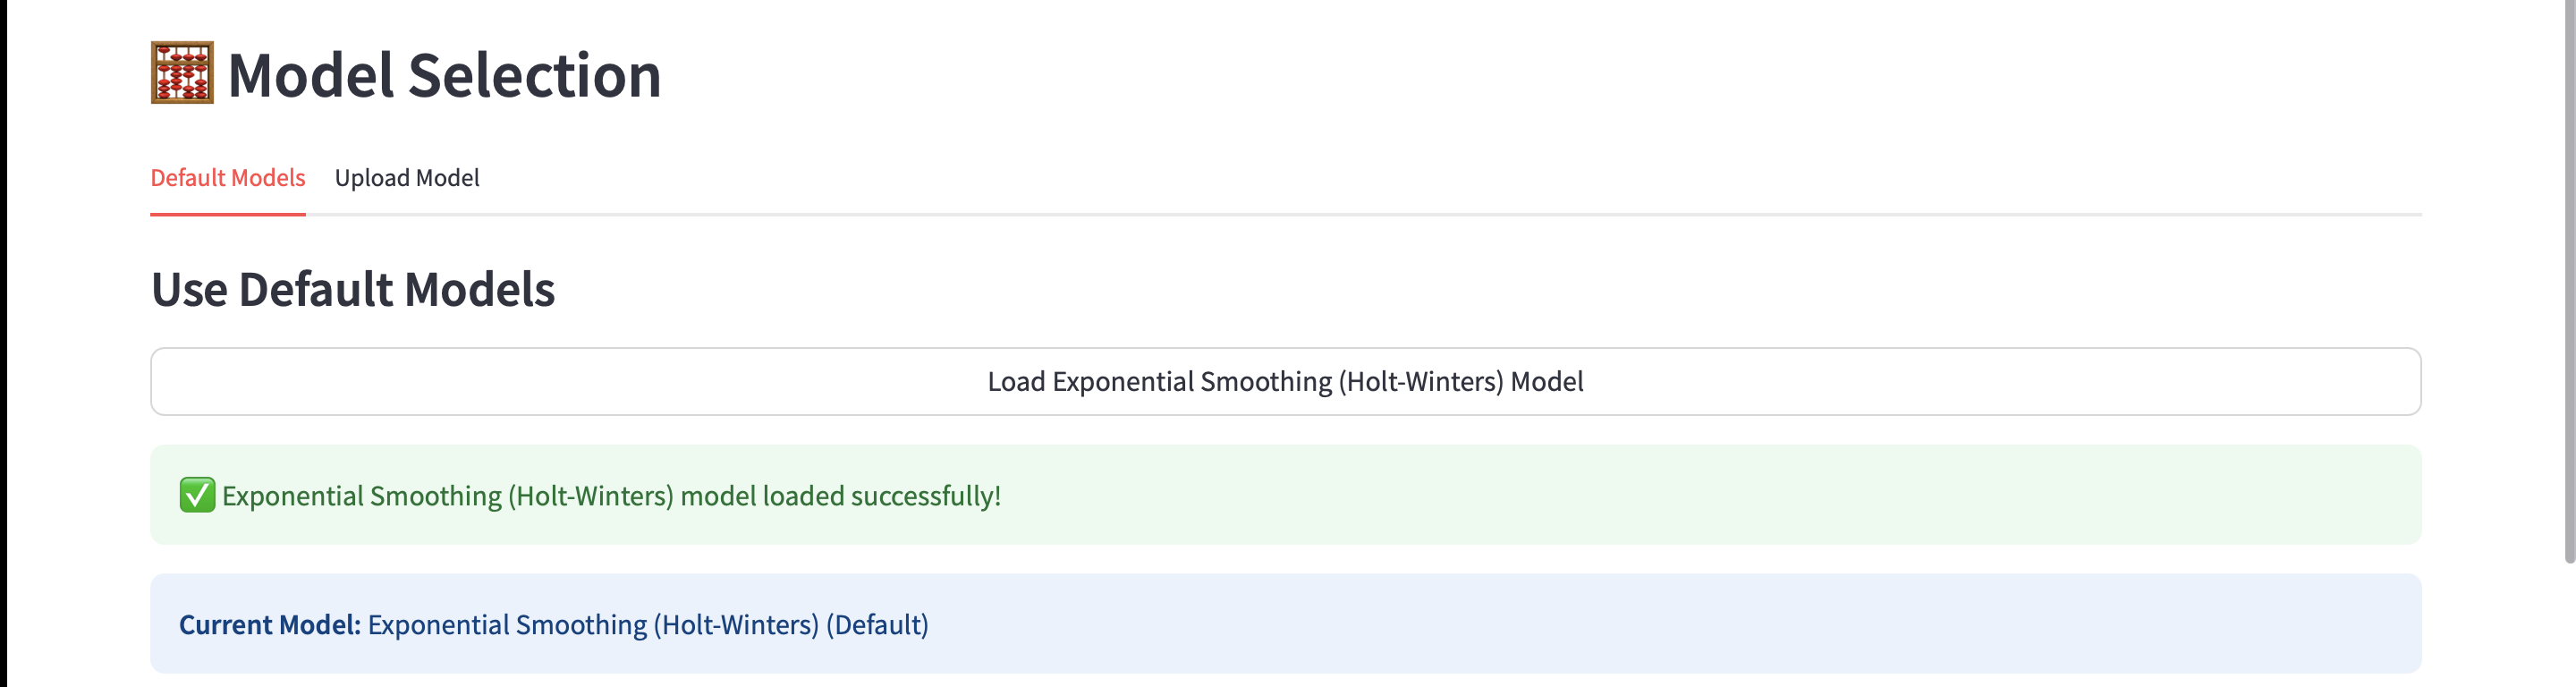
\includegraphics[width=0.9\textwidth]{Images/04GUIAndUserInterface/ModelStatus.png}
    \caption{Current Model Status Display}
    \label{fig:model_status}
\end{figure}

\subsection{Prediction Generation Interface}

\textbf{Forecast Control Section}

\begin{itemize}
    \item \textbf{Primary Action Button}: "Generate 4-Week Forecast" with primary styling
    \item \textbf{Processing Indicator}: Spinner animation during prediction generation
    \item \textbf{Conditional Display}: Only appears when model is properly loaded
\end{itemize}

\begin{figure}[H]
    \centering
    
\includegraphics[width=0.9\textwidth]{Images/04GUIAndUserInterface/PredictionGeneration.png}
    \caption{Prediction Generation Control Interface}
    \label{fig:prediction_generation}
\end{figure}

\subsection{Results Visualization Interface}

\textbf{Interactive Chart Display}

The results section provides comprehensive visualization:

\begin{itemize}
    \item \textbf{Plotly Interactive Chart}: Zoom, pan, and hover capabilities
    \item \textbf{Color-Coded Bars}: Green for positive changes, red for negative
    \item \textbf{Reference Line}: Zero-line for easy positive/negative identification
    \item \textbf{Chart Controls}: Built-in zoom, pan, and reset tools
\end{itemize}

\begin{figure}[H]
    \centering
    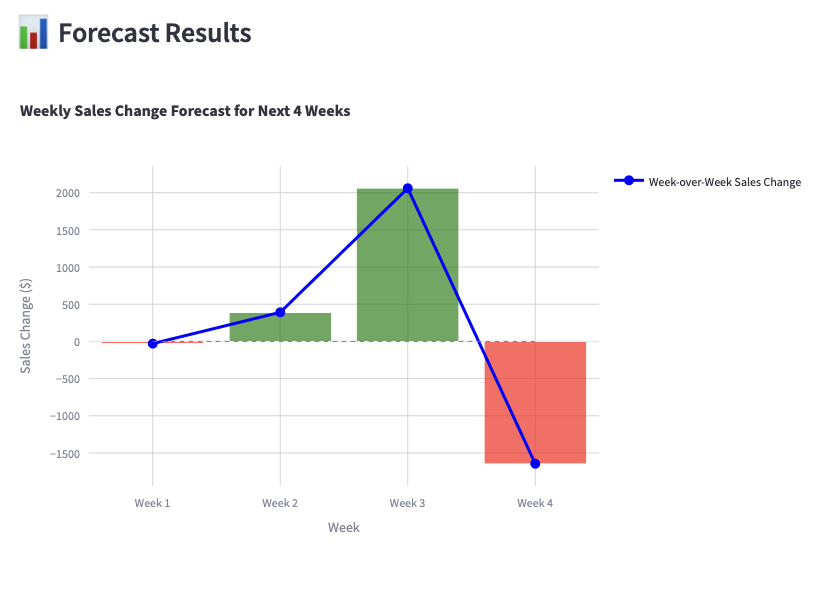
\includegraphics[width=0.9\textwidth]{Images/04GUIAndUserInterface/ResultsVisualization.png}
    \caption{Interactive Results Visualization Interface}
    \label{fig:results_visualization}
\end{figure}

\subsection{Data Table Interface}

\textbf{Formatted Results Table}

\begin{itemize}
    \item \textbf{Color-Coded Values}: Green for positive changes, red for negative
    \item \textbf{Formatted Currency}: Dollar signs and proper decimal formatting
    \item \textbf{Week Labels}: Clear week numbering and date display
    \item \textbf{Responsive Design}: Table adapts to different screen sizes
\end{itemize}

\begin{figure}[H]
    \centering
 %   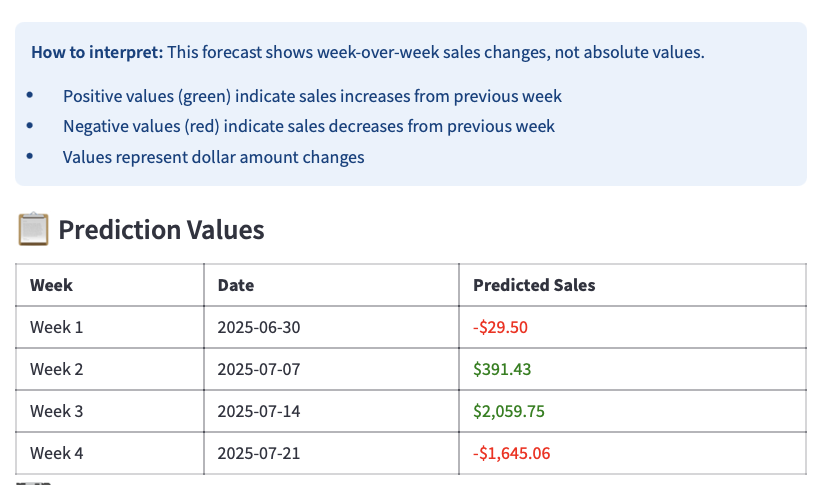
\includegraphics[width=0.9\textwidth]{Images/04ResultsVisualizationGUIAndUserInterface/DataTable.png}
    \caption{Formatted Data Table with Color Coding}
    \label{fig:data_table}
\end{figure}

\subsection{Download and Export Interface}

\textbf{Multi-Format Export Options}

\begin{itemize}
    \item \textbf{Two-Column Layout}: CSV and JSON download buttons
    \item \textbf{File Naming}: Automatic naming with descriptive filenames
    \item \textbf{Format Icons}: Visual indicators for different file types
    \item \textbf{Full-Width Buttons}: Easy-to-click download controls
\end{itemize}

\begin{figure}[H]
    \centering
    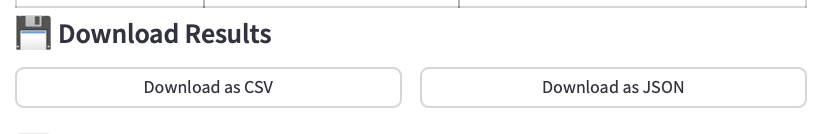
\includegraphics[width=0.9\textwidth]{Images/04GUIAndUserInterface/DownloadInterface.png}
    \caption{Download and Export Interface Options}
    \label{fig:download_interface}
\end{figure}

\section{Common Interface Elements}

\subsection{Navigation and Layout}

\textbf{Consistent Design Patterns}

Both applications share common interface elements:

\begin{itemize}
    \item \textbf{Sidebar Navigation}: Streamlit's built-in navigation structure
    \item \textbf{Section Headers}: Consistent typography and emoji icons
    \item \textbf{Action Buttons}: Uniform styling with primary/secondary distinction
    \item \textbf{Status Messages}: Color-coded success, warning, and error indicators
\end{itemize}

\subsection{Responsive Design}

\textbf{Multi-Device Compatibility}

\begin{itemize}
    \item \textbf{Desktop Optimization}: Full-width layouts with multi-column sections
    \item \textbf{Tablet Adaptation}: Responsive column stacking and button sizing
    \item \textbf{Mobile Support}: Single-column layouts with touch-friendly controls
\end{itemize}

\subsection{Accessibility Features}

\textbf{Inclusive Design Elements}

\begin{itemize}
    \item \textbf{Color Contrast}: High contrast ratios for text readability
    \item \textbf{Alternative Text}: Descriptive alt text for all images and charts
    \item \textbf{Keyboard Navigation}: Full keyboard accessibility for all controls
    \item \textbf{Screen Reader Support}: Semantic HTML structure for assistive technologies
\end{itemize}

\section{Interactive Features}

\subsection{Real-Time Feedback}

\textbf{Dynamic User Experience}

\begin{itemize}
    \item \textbf{Instant Validation}: Real-time file format checking
    \item \textbf{Progress Indicators}: Visual feedback during long operations
    \item \textbf{Status Updates}: Immediate confirmation of user actions
    \item \textbf{Error Prevention}: Input validation before processing
\end{itemize}

\subsection{Chart Interactivity}

\textbf{Advanced Visualization Controls}

\begin{itemize}
    \item \textbf{Hover Information}: Detailed data points on mouse over
    \item \textbf{Zoom Controls}: Mouse wheel and toolbar zoom functionality
    \item \textbf{Pan Navigation}: Click and drag chart movement
    \item \textbf{Reset View}: One-click return to default chart view
\end{itemize}

\section{Interface Customization}

\subsection{Theme and Styling}

\textbf{Visual Customization Options}

\begin{itemize}
    \item \textbf{Light Theme}: Default high-contrast theme for most users
    \item \textbf{Dark Theme}: Available through browser/OS dark mode settings
    \item \textbf{Font Scaling}: Browser zoom support for accessibility
    \item \textbf{Color Preferences}: System-level color scheme integration
\end{itemize}

\subsection{Layout Preferences}

\textbf{User-Controlled Interface Elements}

\begin{itemize}
    \item \textbf{Section Expansion}: Expandable sections for focused workflow
    \item \textbf{Tab Memory}: Interface remembers last selected tabs
    \item \textbf{Window Sizing}: Automatic adaptation to browser window size
\end{itemize}

\section{Interface Best Practices}

\subsection{Optimal Usage Patterns}

\textbf{Recommended Workflow Navigation}

\begin{itemize}
    \item \textbf{Top-to-Bottom}: Follow the natural page flow for optimal experience
    \item \textbf{Tab Completion}: Complete all inputs in a tab before switching
    \item \textbf{Progressive Disclosure}: Use advanced features only after mastering basics
    \item \textbf{Regular Saves}: Download results frequently to prevent data loss
\end{itemize}

\subsection{Performance Optimization}

\textbf{Interface Responsiveness Tips}

\begin{itemize}
    \item \textbf{Browser Choice}: Latest version of Chrome or Firefox recommended for best performance
    \item \textbf{Tab Management}: Avoid having too many browser tabs open
    \item \textbf{Cache Clearing}: Clear browser cache if interface becomes sluggish
    \item \textbf{Network Stability}: Ensure stable internet connection for cloud usage
\end{itemize}

This comprehensive interface documentation provides the foundation for effective system utilization. The next chapter will detail the specific functions and features available in each application.